\documentclass{slide}

\usepackage{tikz}
\usetikzlibrary{arrows}
\usepackage{tabto}
\usepackage{languages}

% \usepackage{pgfpages}
%\setbeameroption{show notes on second screen}

\title{Distributed Systems II}
\subtitle{Software Architecture}
\author{Brae Webb \& Richard Thomas}
\date{\week{6}}

% \titlegraphic {
%     \tweet%
%     {images/mathiasverraes}%
%     {Mathias Verras}%
%     {mathiasverraes}%
%     {There are only two hard problems in distributed systems:  2. Exactly-once delivery 1. Guaranteed order of messages 2. Exactly-once delivery}%
%     {https://twitter.com/mathiasverraes/status/632260618599403520}%
% }

\begin{document}

\maketitle

\point[Distributed Systems Series]{
    \begin{description}
        \item[Distributed I] \highlight{Reliability} and \highlight{scalability} of \highlight{stateless} systems.
        \item[Distributed II] \highlight{Complexities} of \highlight{stateful} systems.
        \item[Distributed III] \highlight{Hard problems} in distributed systems.
    \end{description}
}

\point[Distributed Systems Series]{
    \begin{description}
        \item[Distributed I] {\color{gray}Reliability and scalability of stateless systems.}
        \item[Distributed II] \highlight{Complexities} of \highlight{stateful} systems.
    \item[Distributed III] {\color{gray}Hard problems in distributed systems.}
    \end{description}
}

\point[Previously in CSSE6400\dots]{
\begin{center}
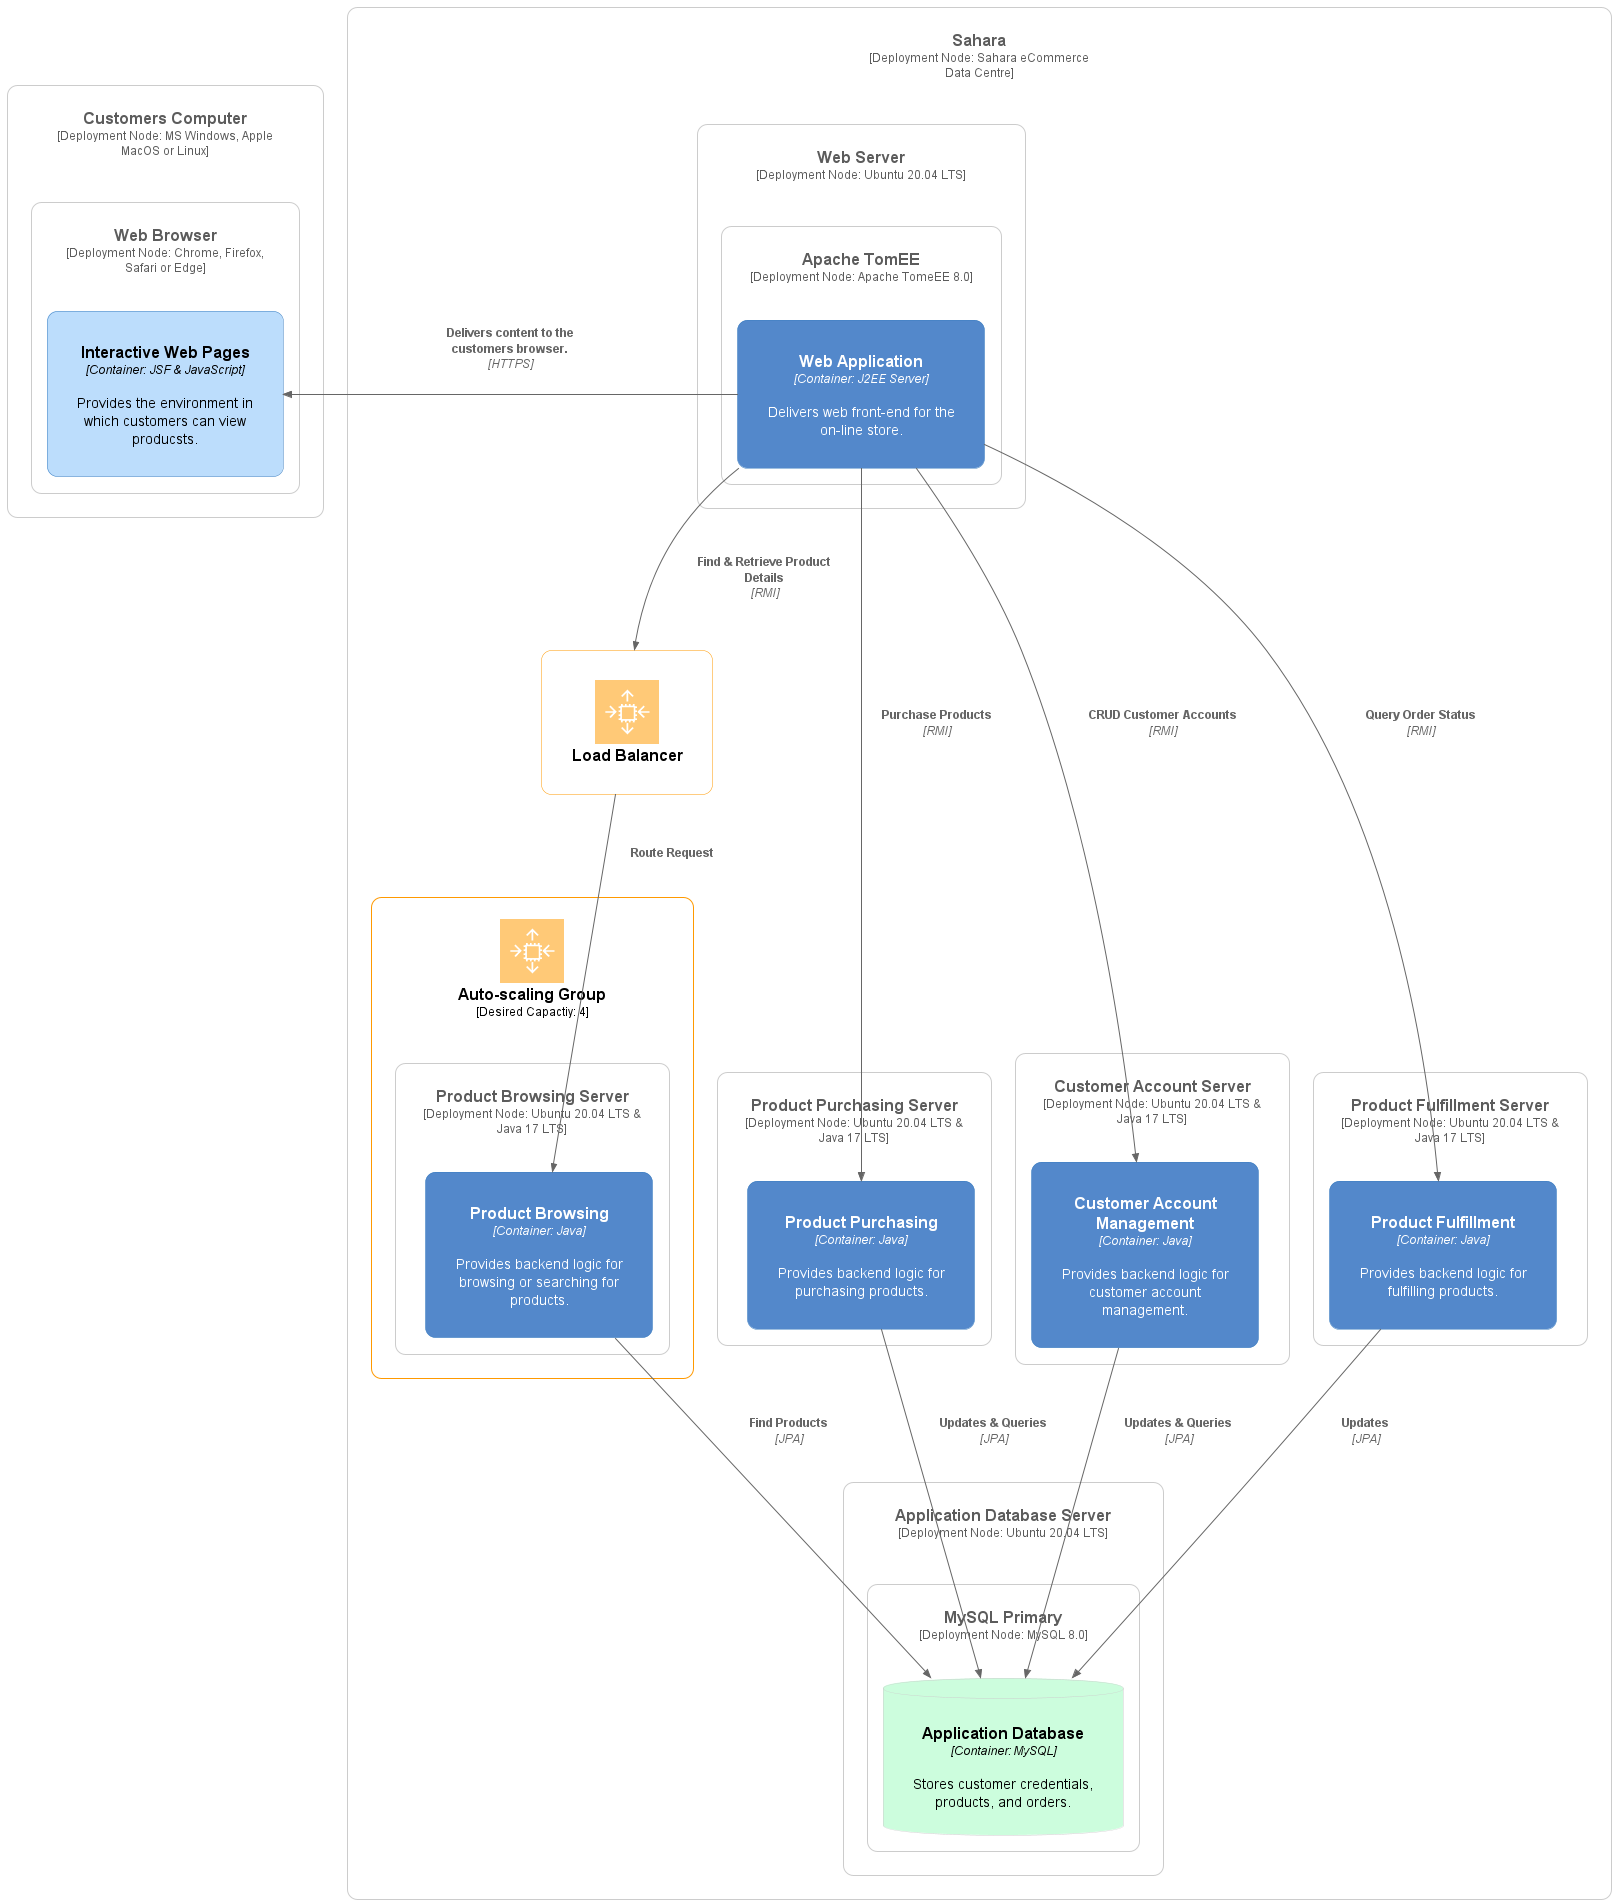
\includegraphics[width=0.8\textheight]{diagrams/SaharaScaled}
\end{center}
}
\note[itemize]{
    \item We scaled a stateless service.
    \item Stateless: Services don't require persistent data \highlight{between} requests.
    \item Persistent state is saved in the database.
    \item This is normally easy to do.
}

\question{What is the \highlight{problem}?}
\note{The database}

\point[Database]{
\begin{center}
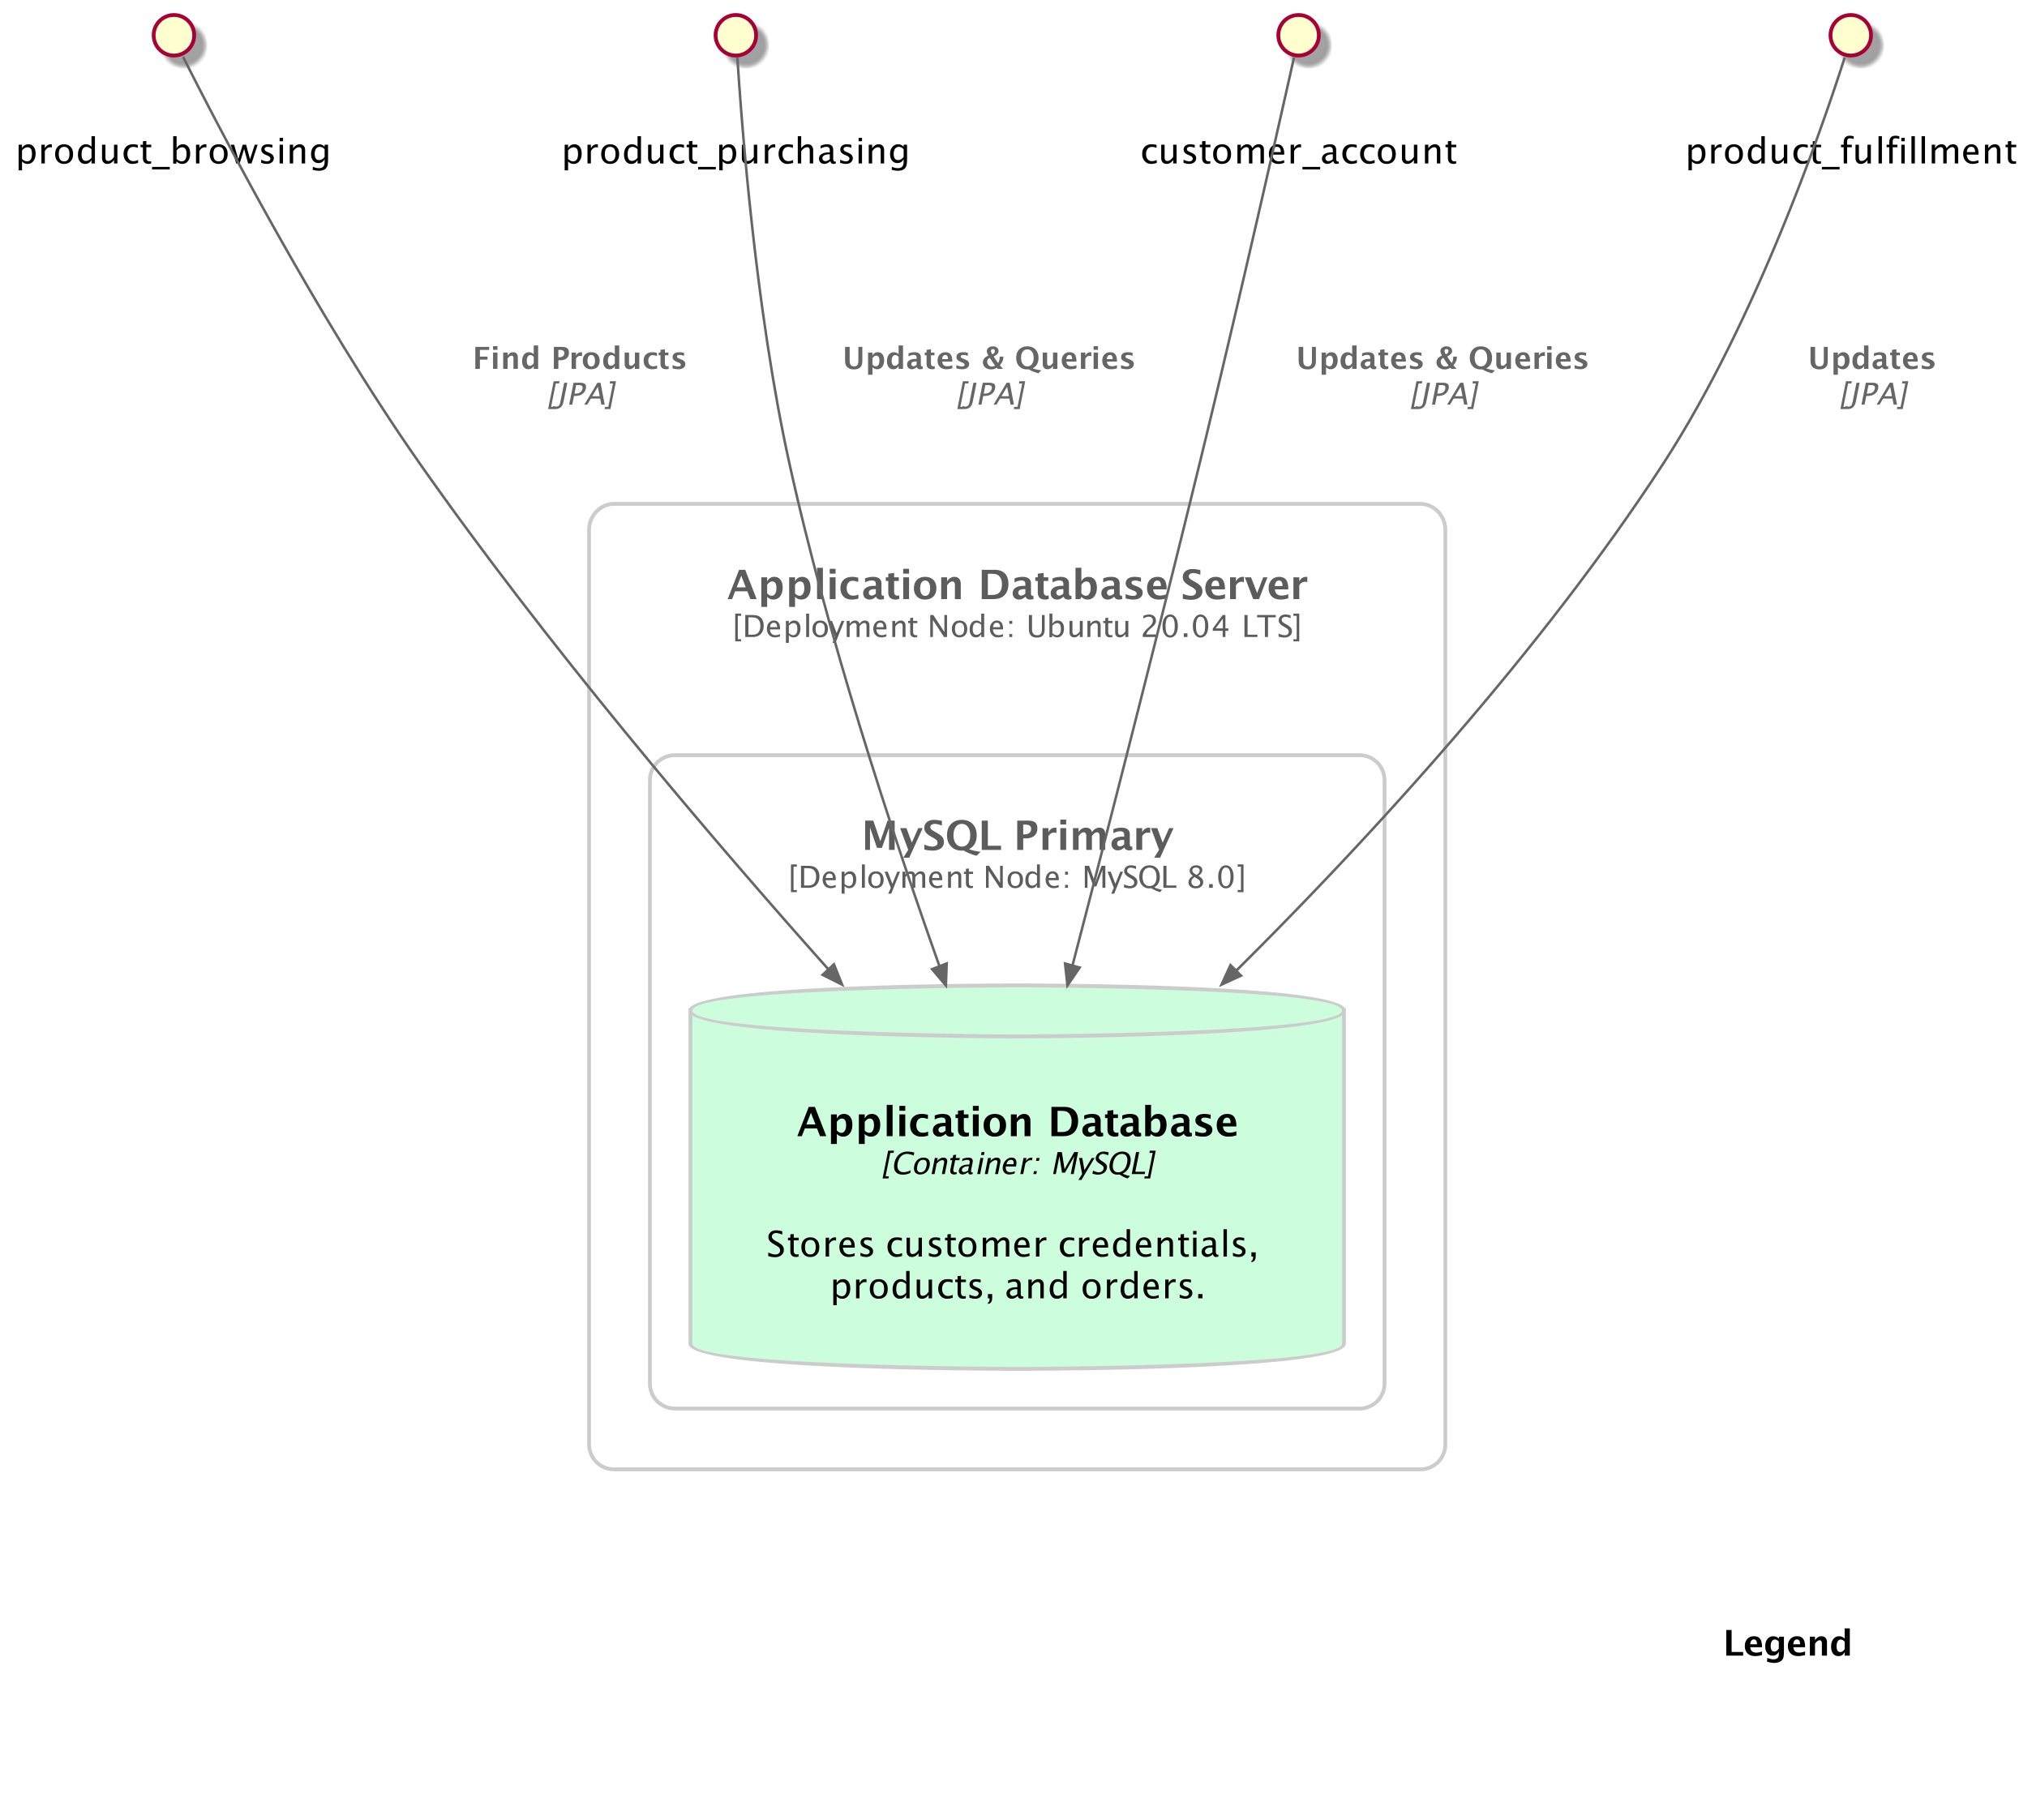
\includegraphics[width=\textheight]{diagrams/FocusDB}
\end{center}
}
\note[itemize]{
    \item Database has state, persistent data.
    \item This is much harder to scale.
}

\point[Disclaimer]{This is \highlight{not} a database course.}

\image{images/infs3200}
\note{This is a database course.}


%%%%%%%%%%%%%%%
% Replication %
%%%%%%%%%%%%%%%
\questionanswer{How do we fix database scaling issues?}{
    \begin{itemize}[<+(1)->]
        \item
        \only<5->{\highlight{Replication}}
        \only<-4>{Replication}
        \item Partitioning
        \item Independent databases
    \end{itemize}
}

\question{What is \highlight{replication}?}

\definition{Replication}{
    Data copied across multiple different machines.
}

\image{diagrams/Replication}

\definition{Replica}{
    Database node which stores a copy of the data.
}

\questionanswer{What are the advantages of \highlight{replication}?}{
    \begin{itemize}[<+(1)->]
        \item \highlight{Scale} our database to cope with higher loads.
        \item Provide \highlight{fault tolerance} from a single instance failure.
        \item Locate instances \highlight{closer to end-users}.
    \end{itemize}
}
\note[itemize]{
    \item Scalability
    \item Reliability
    \item Performance
}

\question{How do we replicate our data?}
\note[itemize]{
    \item Easy without updates, just copy it.
    \item Updates, or writes, must \highlight{propagate} changes.
}

\point[First approach]{Leader-Follower Replication}

\image{diagrams/LeaderFollower}
\note[itemize]{
    \item Leader-Follower is the most common implementation.
    \item Multiple followers, only \textit{one} leader.
}

\point[Leader-based Replication]{
    \begin{description}[<+->]
        \item[On write] Writes sent to \textit{leader}, change is propagated via change stream.
        \item[On read] Any \textit{replica} can be queried. 
    \end{description}
}

\image{diagrams/LeaderFollowerSpread}
\note[itemize]{
    \item Built-in to PostgreSQL, MySQL, MongoDB, RethinkDB, and Espresso.
    \item Can be added to Oracle and SQL Server.
}

\point[Propagating changes]{
    \highlight{Synchronous} vs. \highlight{Asynchronous}
}

\image[height=\textheight]{diagrams/Sync}
\note{Synchronous update.}

\image[height=\textheight]{diagrams/Async}
\note{Asynchronous update.}

\image[height=\textheight]{diagrams/SyncVsAsync}
\note[itemize]{
    \item What could go wrong here?
    \item \textit{Follower1} can get out of sync with \textit{Follower2}.
    \item Following material deals with \textit{leader} or a \textit{replica} going down.
}

\point[Synchronous Propagation]{
\begin{itemize}[<+->]
    \item Writes must propagate to \highlight{all followers} before being successful.
    \item \highlight{Any} replica goes down, \highlight{all} replicas are un-writeable.
    \item Writes must \highlight{wait} for propagation to \highlight{all} replicas.
\end{itemize}
}

\point[Asynchronous Propagation]{
\begin{itemize}[<+->]
    \item Writes \highlight{don't} have to \highlight{wait} for propagation.
    \item If the leader goes down before propagating, the \highlight{write is lost}.
    \item Replicas can have out-dated or \highlight{stale} data.
\end{itemize}
}

% \todo{There could be content here about handling node failures}

% \point[When things go wrong]{
%     Handling outages
% }

% \point{Follower failure}

% \point{Leader failure}

\definition{Replication Lag}{
    The time taken for replicas to update \highlight{stale} data.
}

\image{diagrams/ReplicationLag}
\note{\textit{Replication Lag}: Time it takes for the product name change to update across \highlight{all} followers.}

\image[height=\textheight]{diagrams/AsyncLag}
\note{The purple lifeline bar is \textit{replication lag}.}

\point[Eventually, all replicas must become consistent]{
    The system is \highlight{eventually consistent}.
}
\note[itemize]{
    \item If writes stop for long enough.
    \item Eventually is intentionally \highlight{ambiguous}.
}

\point[Eventual Consistency]{Problems?}

\begin{frame}
\begin{center}
\tweet%
{images/braewebb}%
{Brae Webb}%
{braewebb}%
{}%
{}%
\note[item]<1->{Read user details.\vspace{1em}}

\only<2->{
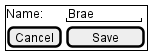
\includegraphics[width=0.3\textwidth]{diagrams/ReadYourWrites}
}
\note[item]<2->{Decide I don't like my name.\vspace{1em}}
\note[item]<2->{Update name.\vspace{1em}}

\only<3->{
\tweet%
{images/braewebb}%
{Brae Webb}%
{braewebb}%
{}%
{}%
}
\note[item]<3->{Read user details.}

\end{center}
\end{frame}

\image{diagrams/ReadYourWritesExample}
\note[itemize]{
    \item Typical interaction in simple Leader-Follower replication.
    \item Write is to \highlight{leader}.
    \item Read is from \highlight{follower}.
    \item \textit{Replication lag} means reading a field immediately after updating it \highlight{may} lead to reading \highlight{stale} data.
}

\definition{Read-your-writes Consistency}{
    Users always see the updates that \highlight{they have made}.
}
\note{Doesn't care what other users see.}

\begin{frame}
\begin{center}
\only<1->{
\tweet%
{images/braewebb}%
{Brae Webb}%
{braewebb}%
{My fist post}%
{}%
}
\note[item]<1->{Misspell a tweet.\vspace{1em}}

\only<2->{
\tweet%
{images/braewebb}%
{Brae Webb}%
{braewebb}%
{My first post}%
{}%
}
\note[item]<2->{Correct spelling, and I see my \textit{updated} tweet.\vspace{1em}}

\only<3->{
\tweet%
{images/braewebb}%
{Brae Webb}%
{braewebb}%
{My fist post}%
{}%
}
\note[item]<3->{Other users may still see \textit{stale}, misspelt post.}
\end{center}
\end{frame}

\image{diagrams/MonotonicReads}
\note[itemize]{
    \item Go through each step in sequence.
    \item Step 6: 3rd view post, gets \highlight{old value}.
}

\definition{Monotonic Reads}{
    Once a user reads an updated value, they don't later see the old value.
}
\note{User doesn't travel back in time.}

% \point{Consistent Prefix Reads}
% \todo{Consistent Prefix Example}

\point[Summary]{
\begin{itemize}
    \item Leader-follower databases allow \highlight{reads to scale} more effectively.
    \item Asynchronous propagation weakens consistency to \highlight{eventually consistent}.
    \item Leader-follower databases still have a \highlight{leader write bottle-neck}.
\end{itemize}
}

\point[Second approach]{Multi-leader Replication}

\image[height=\textheight]{diagrams/MultiLeader}
\note[itemize]{
    \item Application can be partitioned to perform certain types of writes to a specific leader.
    \item Reads are from replicas, as with Leader-Follower replication.
}

\point[Why multi-leader?]{
\vspace{1em}
\begin{itemize}[<+->]
    \item If you have multiple leaders,
          you can write to any,
          allowing \highlight{writes to scale}.
          \vspace{1em}
    \item A leader going down doesn't prevent writes,
          giving \highlight{better fault-tolerance}.
\end{itemize}
}
\note[itemize]{
    \item Available via extensions in most databases, often not supported natively.
    \item Best to avoid where possible.
    \item Example: Globally distributed data centres.
}

% \point[Multi-leader Replication]{Use Cases}
% \note[itemize]{
%     \item Multiple datacenters
%     \item Offline writing
% }

\questionanswer{What might go wrong?}{Write conflicts}
\note{Conflict needs to be \highlight{resolved}.}

\image{diagrams/WriteConflict}
\note[enumerate]{
    \item Fulfilment centre finds faulty pillow and decreases inventory.
    \item Customer orders 20 pillows, what they saw as the number available.
    \item -1 Pillows?
    \item How do we resolve this?
}

\point[Where possible]{Avoid write conflicts}

\image{diagrams/AvoidWriteConflict}
\note{Requires application to ensure all writes to a field/table/shard are via the \highlight{same} leader.}

\point[Where impossible]{Convergence}

\point[Convergence Strategies]{
\begin{itemize}[<+->]
    \item Assign each \highlight{write} a unique ID.
    \item Assign each \highlight{leader replica} a unique ID.
    \item Custom resolution logic.
\end{itemize}
}
\note{Yes, this can be \highlight{challenging}.}

\image[height=\textheight]{diagrams/ResolveWriteConflict}

\point[Resolving Conflicts]{
\vspace{1em}
\begin{description}
    \item[On Write] When a conflict is first noticed, take proactive resolution action.
    \vspace{1em}
    \item[On Read] When a conflict is next read, ask for a resolution.
\end{description} 
}
\note[itemize]{
    \item Bucardo allows a perl script for on write resolution.\vspace{1em}
    \item CouchDB prompts reads to resolve the conflict.
}

% \point[Cutting Edge]{Automatic Conflict Resolution}

\point[Third Approach]{Leaderless Replication}
\note[itemize]{
    \item Early distributed databases were leaderless.
    \item Resurgance after Amazon created Dynamo.
    \item Dynamo is an internal service and \highlight{not} DynamoDB.
    \item Riak, Cassandra, and Voldemort are leaderless databases.
}

\image{diagrams/Leaderless}
\note{Reads and writes can be written to any node.}

\point[How do they work?]{
    Each read/write is sent to \highlight{multiple} replicas.
}

\image{diagrams/LeaderlessExampleWrite}
\note{Leaderless Write}

\image{diagrams/LeaderlessExampleRead}
\note{Leaderless Read: At least one of the reads has the updated value.}

\point[How are changes propagated?]{
    \begin{itemize}[<+->]
        \item Read Repair
        \note[item]<1->{Read Repair: Client detects stale data on read and writes updated data to that replica.\vspace{1em}}
        \item Anti-Entropy Process
        \note[item]<2>{Anti-Entropy Process: Background process looks for stale or missing data and updates replicas.}
    \end{itemize}
}

\question{How do we know it's consistent?}

\image{diagrams/LeaderlessExampleBad}
\note{Reading from a single replica means we can't know if data is stale or inconsistent.}

\questionanswer{How do we know it's consistent?}{
    Quorum Reads and Writes
}

\definecolor{eq1}{RGB}{116, 137, 227}
\definecolor{eq2}{RGB}{227, 116, 137}

\point[Quorum Consistency]{
\only<1>{
\begin{equation*}
\textcolor{eq1}{w} + \textcolor{eq2}{r} > \textcolor{focus}{n}
\end{equation*}
}
\only<2>{
\begin{equation*}
\textcolor{eq1}{2} + \textcolor{eq2}{2} > \textcolor{focus}{3}
\end{equation*}
}
\only<3>{
\begin{equation*}
\textcolor{eq1}{1} + \textcolor{eq2}{3} > \textcolor{focus}{3}
\end{equation*}
}

\Large
\begin{description}
    \item[$\textcolor{focus}{n}$] total replicas
    \item[$\textcolor{eq1}{w}$] amount of replicas to {\color{eq1}\textsl{write}} to
    \item[$\textcolor{eq2}{r}$] amount of replicas to {\color{eq2}\textsl{read}} from
\end{description}
}
\note{Nodes read from must overlap with the nodes written to.}

\begin{frame}
\begin{center}
    \begin{tikzpicture}
        \node[anchor=south west,inner sep=0] at (0,0.5) {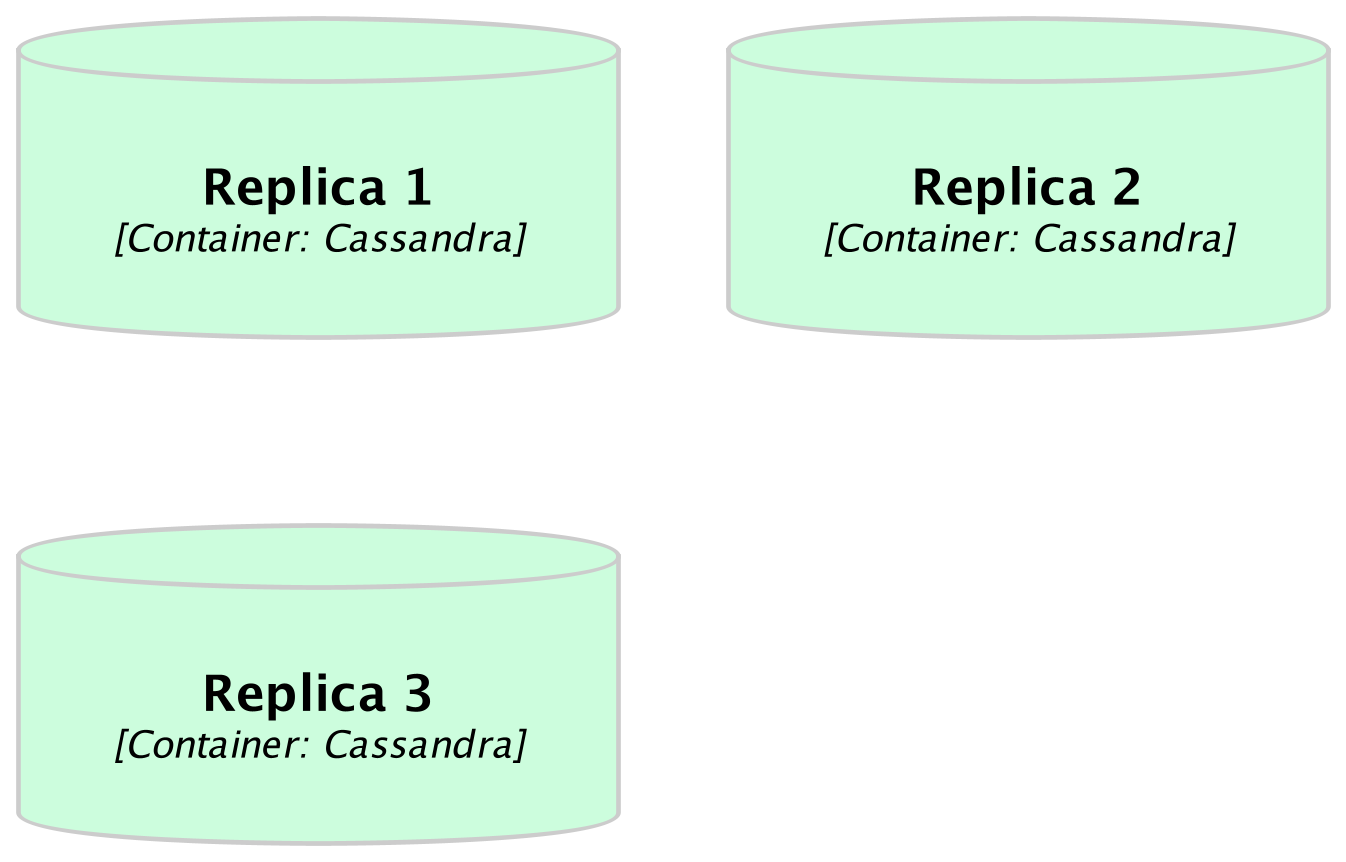
\includegraphics[width=0.8\textwidth]{diagrams/LeaderlessQuorum}};
        \draw[eq1,ultra thick,rounded corners] (0,0) rectangle (5.5,8.2);
        \draw[eq2,ultra thick,rounded corners] (0,4.5) rectangle (11.5,8.2);
        \draw[focus,ultra thick,rounded corners] (-0.1,-0.1) rectangle (11.6,8.3);
        \node at (8.5,3.5) {
            $\textcolor{focus}{n}$ total replicas
        };
        \node at (8.5,2.5) {
            $\textcolor{eq1}{w}$ amount of replicas to {\color{eq1}\textsl{write}} to
        };
        \node at (8.5,1.5) {
            $\textcolor{eq2}{r}$ amount of replicas to {\color{eq2}\textsl{read}} from
        };
    \end{tikzpicture}
\end{center}
\end{frame}
\note[itemize]{
    \item Graphical representation of previous equation. \vspace{3mm}
    \item \textcolor{eq2}{\textbf{Orange}} inner group (\highlight{reads}), overlaps with \\ 
           \textcolor{eq1}{\textbf{Blue}} inner group (\highlight{writes}). \vspace{3mm}
    \item Showing how reads overlap writes via a quorum.
}

\questionanswer{What about write conflicts?}{Same problem as with Multi-leader replication.}

\image{diagrams/LeaderlessExampleWriteConflict1}
\note{
  Same scenario as before:
  \begin{enumerate}
    \item Customer queries how many pillows are available.
    \item Retrieves 20.
  \end{enumerate}
}

\image{diagrams/LeaderlessExampleWriteConflict2}
\note{Same scenario as before:}
\note{
  Same scenario as before:
  \begin{enumerate}
    \item Fulfilment centre finds faulty pillow and decreases inventory.
    \item Customer orders 20 pillows, what they saw as the number available.
    \item -1 Pillows?
    \item How do we resolve this?
  \end{enumerate}
}

\point[Summary]{
\begin{itemize}[<+->]
    \item \highlight{Replication} copies data to multiple replicas.
    \item \highlight{Leader-based} replication is most common and simpliest.
    \item Replication introduces \highlight{eventual consistency}.
    \item \highlight{Multi-leader} replication scales writes as well as reads but introduces \highlight{write conflicts}.
    \item \highlight{Leaderless} replication is another approach which keeps the problems of multi-leader.
\end{itemize}
}


%%%%%%%%%%%%%%%%
% Partitioning %
%%%%%%%%%%%%%%%%
\questionanswer{How do we fix database scaling issues?}{
    \begin{itemize}
        \item 
        \only<-2>{\highlight{Replication}}
        \only<3->{Replication}
        \item 
        \only<3->{\highlight{Partitioning}}
        \only<-2>{Partitioning}
        \item Independent databases
    \end{itemize}
}

\definition{Partitioning}{
    Split the data of a system onto multiple nodes. \\These nodes are \highlight{partitions}.
}
\note{Also called shards, regions, tablets, etc.}

\image{diagrams/Partitioning}
\note[itemize]{
    \item Pioneered in the 1980s.
    \item Allow scalability of large data, not just large load.
    \item Partitioning is normally combined with replication.
}

\question{How should we decide which data is stored where?}

\image[height=\textheight]{diagrams/PartitioningExample}
\note{An example partitioning based on primary key, student ID.}

\questionanswer{What is the problem with this?}{
    Over time some partitions become inactive,
    while others receive almost all load.
}

\questionanswer{
    How should we decide which data is stored where?
}{
    Maximize spread of requests, avoiding \highlight{skewing}.
}

\questionanswer{Have we seen this before?}{Hashing?}
\note{Hash tables hash entries to maximize the spread between buckets.}

\questionanswer{What is the problem with this?}{
    Range queries are inefficient, i.e. get all students between s4444444 and s4565656.
}

\question{How do we route queries?}
\note{Unlike stateless, only one node can process queries.}

\point[Query-insensitive Load Balancer]{
    Randomly route to any node, responsibility of the node to re-route to the correct node.
}

\image{diagrams/PartitioningLB1}

\point[Query-sensitive Load Balancer]{
    A load balancer which understands which queries should be forwarded to which node.
}

\image[height=\textheight]{diagrams/PartitioningLB2}


\point[Client-aware Queries]{
    Place the responsibility on clients to choose the correct node.
}

\image{diagrams/PartitioningLB3}

\point[Summary]{
\begin{itemize}[<+->]
    \item \highlight{Partitioning} splits data across multiple nodes.
    \item A \highlight{consistent method} to chose which node is required.
    \item Partitioning by \highlight{primary key} can create \highlight{skewing}.
    \item Partitioning by \highlight{hash} makes range queries less efficient.
    \item Three approaches to \highlight{routing requests}.
\end{itemize}
}

\point[Disclaimer]{We have ignored the hard parts of replication.}


%%%%%%%%%%%%%%%%%%%%%%%%%%%%%
% Isolation (foreshadowing) %
%%%%%%%%%%%%%%%%%%%%%%%%%%%%%
\questionanswer{How do we fix database scaling issues?}{
    \begin{itemize}
        \item Replication
        \item 
        \only<-2>{\highlight{Partitioning}}
        \only<3->{Partitioning}
        \item 
        \only<3->{\highlight{Independent databases}}
        \only<-2>{Independent databases}
    \end{itemize}
}

%\point{Distributed state creates a lot of \highlight{complexity}}
%\note{And when programmers have complexity, they create bugs}

%\point[When programmers are faced with complexity]{
%    They create \highlight{abstractions}
%}

%\point[One key database abstraction]{Transactions}
%\note{Introduced by IBM System R in 1975}

%\definition{Transaction}{A group of operations performed as if they were one.}
%\note{What does as if it were one mean?}

%\begin{frame}{ACID}
%    \Huge
%\begin{description}
%    \item[A] tomic
%    \item[C] onsistent
%    \item[I] solated
%    \item[D] urable
%\end{description}
%\end{frame}

%\point[The pushback]{
%    NoSQL and microservice architectures pushed back against transactions.
%}
%\note[itemize]{
%    \item Transactions were used fairly universally for a long time.
%    \item Push back occurred when people decided they weren't scalable.
%}

%\point[For more on transactions]{
%    \centering \youtubevideo{images/transactions}{https://www.youtube.com/watch?v=5ZjhNTM8XU8}
%}

\point[Summary]{
    \begin{itemize}[<+->]
        \vspace{4mm}
        \item Replications
        \begin{itemize}
            \Large
            \item Leader-based, multi-leader, and leaderless
            \item Eventual consistency
            \item Write conflicts
        \end{itemize}
        \vspace{2mm}
        \item Partitioning
        \begin{itemize}
            \Large
            \item Consistent method to pick nodes for data
            \item Avoiding skewing
        \end{itemize}
%        \vspace{2mm}
%        \item Transactions
%        \begin{itemize}
%            \Large
%            \item ACID properties
%            \item Pushback causing headaches
%        \end{itemize}
    \end{itemize}
}

% \references{articles,books}

\end{document}
